\chapter{Review of MDO architecture}
\markboth{Review of MDO architecture}{Review of MDO architecture}
\label{app:mdo_rev}


\section{An introduction to the MDO}
\label{sec:app2_mdo_intro}
The multidisciplinary design optimization (MDO), as defined by Martins and Lambe~\cite{bib:martins_mdo}, is a ``field of engineering that focuses on the use of numerical optimization for the design of systems that involve a number of disciplines and subsystems''.
The main motivation behind MDO is the multidisciplinarity: generally, a system is driven by different disciplines at same time, and thus the interaction between them becomes even more important than the performance of an individual discipline. 
To take into account these interactions, MDO requires a well posed mathematical formulation. 
Solving the MDO problem early in the design process helps designers to improve the design, reducing at same time computational cost: it is then a powerful tool, that has become more and more important for engineers.  

MDO origins can be traced back to '60 years, when Haftka~\cite{bib:haftka_1973, bib:haftka_1975, bib:haftka_1977, bib:haftka_1979} and Schmit~\cite{bib:schmit_1960, bib:schmit_1965, bib:schmit_1981, bib:schmit_1984} started to extend their experience in the structural optimization to other disciplines. 
Throughout decades, it has been successfully applied to a large variety of engineering problems: in the aerospace field, it has been used to solve the aeroelastic optimization, where structure, aerodynamics and control are strongly coupled~\cite{bib:ashley, bib:green, bib:grossman_1988, bib:grossman_1990, bib:livne_1990, bib:livne_1999, bib:jansen_2010, bib:ning}, rotorcraft design~\cite{bib:ganguli}, wind turbines design~\cite{bib:fuglsang}, spacecraft and satellite design~\cite{bib:braun, bib:hwang_satellite}, and even full aircraft design~\cite{bib:kroo, bib:manning, bib:antoine, bib:henderson, bib:alonso}.  
It is to underline that the examples given vary from low fidelity problems, with limited number of design variables, to problems based on high fidelity, with thousands of variables involved. 
In general, low fidelity problems involve large number of disciplines, meanwhile high fidelity problems are limited to one/two disciplines, due to the computational time required. 
In recent years, thanks to the improvements in computational science and the new resources available, the major interest of MDO application is found within the high fidelity optimization: an example has already been given in Chapter~\ref{chap1:state_art}, with respect to the BWB optimization carried out by Lyu and Martins~\cite{bib:lyu}. 

The MDO process is mainly defined by its architecture, which is the ensemble of problem formulation and organization strategy (order of disciplines, model used, $\cdots$). 
The MDO architecture, then, not only contains the algorithm used to find an optimal solution, but also the models that characterize the problem: replacing a low fidelity method with an higher one for an individual discipline will change the architecture, since it will lead to a different optimal solution, even with the same algorithm used. 

Conceptually, many different architectures can be used to solve a given design problem, but not all of them will do the optimization with the same efficiency~\cite{bib:tedford, bib:martins_2009, bib:padula}: Fig.~\ref{fig:mdo_benchmarking} reports the results of a benchmarking of different MDO architectures, carried out by Tedford and Martins, clearly showing that there are some architectures that work well than others on a given design problem.
\begin{figure}[!h]
	\centering
	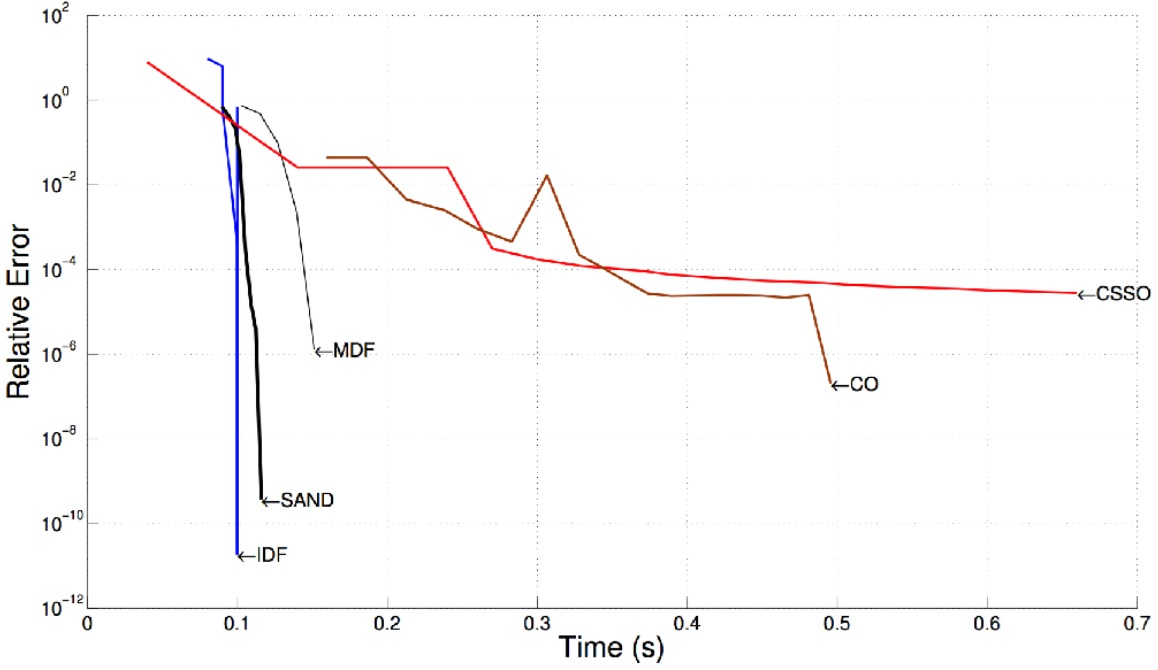
\includegraphics[keepaspectratio, width=0.8\linewidth]{images/app_mdo/mdo_arch_benchmarking.jpg}
	\caption{Comparison between the relative error using different MDO architectures on a given design problem~\cite{bib:tedford}.}
	\label{fig:mdo_benchmarking}
\end{figure}

There are two family or MDO architectures: monolithic~\cite{bib:cramer} and distributed~\cite{bib:dantzig, bib:benders}. 
The first ones are tailored to solve a single problem optimization, meanwhile the second ones customize the problem and multiple optimization subproblems are solved with subsets of variables and constraints. 
Generally, the aircraft design problem is a fully coupled problem, where disciplines exchange information each others. 
As example, the aerodynamics and the structure sizing are strongly correlated: the aerodynamic loads are the main one to consider in the structural design. 
Thusthere is no particular interest in optimizing each discipline separately, in a collaborative manner, but it is more relevant to have a top level optimizer that involves each discipline, as in monolithic architecture. 
For this reason, further details are provided only for this class of architectures. 
Nevertheless, it may be possible, for any reason, to have an aircraft design problem in which it is of interest to optimize disciplines separately, with a distributed architecture; then small notes on this class are provided by the end, following the division done by Martins and Lambe~\cite{bib:martins_mdo}. 

Further classification can be done based on the algorithm used. 
In particular, there are two main categories of algorithm: global or gradient-free~\cite{bib:conn, bib:zadeh} and gradient based~\cite{bib:hwang_unif}. 
The first solves the problem in a "global" sense, that is they explore a certain number of points contained in a prescribed design of experiment to finally get the optimum one. 
So the result is always the global minimum point; the main drawback is that they require a large number of points, and thus the computational cost may be high. 
On the other side, gradient based algorithms use the derivatives information to find the direction towards the minimum point, as graphically shown in Fig.~\ref{fig:grad_based_scheme}. 
\begin{figure}[!h]
	\centering
	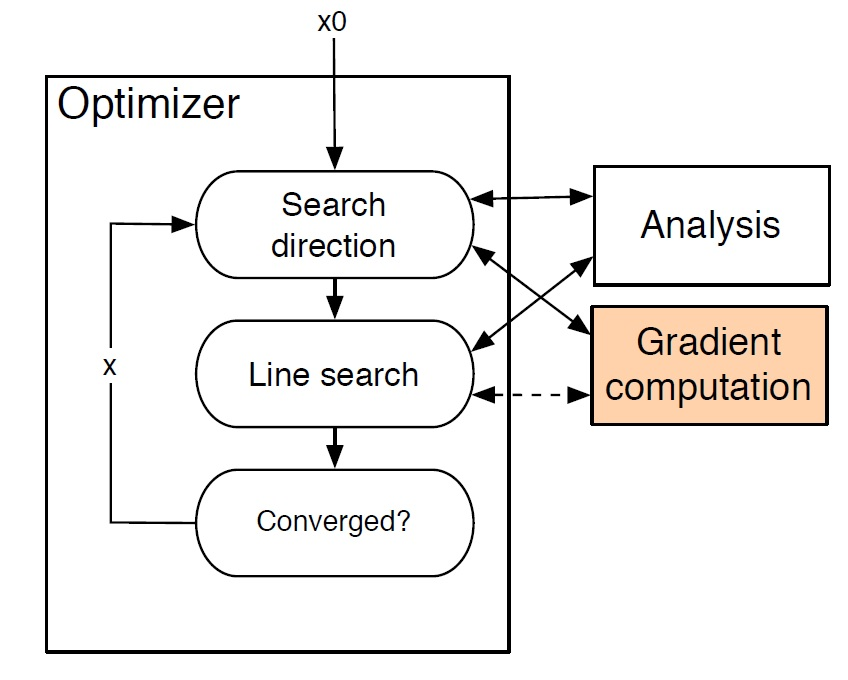
\includegraphics[keepaspectratio, width=0.5\textwidth]{images/app_mdo/grad_based_algo.jpg}
	\caption{Gradient based algorithm scheme for MDO problems~\cite{bib:martins_2014}.}
	\label{fig:grad_based_scheme}
\end{figure}
The gradient-based algorithms are more complicated to code than the gradient-free, since they require derivatives computation; also, they may lead to a different result because they may find a local minimum early in the process. 
However, if the gradients can be efficiently computed, the computational cost may be drastically reduced because of the limited number of iterations required~\cite{bib:zingg}. 
In his Ph.D. thesis, Hwang set up a framework to compute analytic derivatives, using direct or adjoint method, for large-scale problems, called MAUD (Modular Analysis and Unified Derivatives)~\cite{bib:hwang_omdao}. 
This procedure has been later used on a satellite optimization test case~\cite{bib:hwang_satellite}, with promising results, and finally coded in OpenMDAO, an open-source optimization framework~\cite{bib:gray_omdao}. 

Before to proceed on an overview of the available architectures, some notations have to be introduced. 
Here it is used the terminology and the mathematical notation used by Martins and Lambe~\cite{bib:martins_mdo}, which is summed up in Table~\ref{tab:mdo_math_notation}, with the only difference that the underlining denotes a vector, \textit{i.e.} $x$ represents a generic design variable, meanwhile $\underline{x}$ is a vector containing all the design variables.
\begin{table}[!h]
	\centering
	\begin{tabular}{l l}
		\hline
		\textbf{Symbol} & \textbf{Definition} \\
		\hline
		$\underline{x}$ & Vector of design variables \\
		$\underline{y}$ & Vector of coupling variables (outputs from a discipline analysis) \\
		$\underline{\bar{y}}$ & Vector of state variables (variables used inside only one discipline analysis) \\
		$f$ & Objective function \\
		$\underline{c}$ & Vector of design constraints \\
		$\underline{c}^c$ & Vector of consistency constraints \\
		$\mathcal{R}$ & Governing equations of a discipline analysis in residual form  \\
		$N$ & Number of disciplines \\
		$()^{(0)}$ & Initial values of design variables \\
		$()_0$ & Functions of variables that are shared by more than one discipline \\
		$()_i$ & Functions of variables that apply only to discipline $i$ \\
		$()^*$ & Functions of variables at their optimal value \\
		$\tilde{()}$ & Approximations of a given function or vector of functions \\
		$()^t$ & Independent copies of variables distributed to other disciplines \\
		\hline 
	\end{tabular}
	\caption{Mathematical notation for MDO problem formulations, given by Martins and Lambe~\cite{bib:martins_mdo}.}
	\label{tab:mdo_math_notation}
\end{table}
The first parameter to define is the objective function $f$, which is the parameter to be minimized at the end of the optimization problem. 
A design variable is a parameter that is always under the control of the optimizer, that is the parameter the objective function depends on. 
To differentiate local design variables, that concern a single discipline, to the shared one, the subscript $()_i$ and $()_0$ are used. 
The same convention applies to state variables and constraints. 
$\bar{y}$ denotes generally a state variable, that is the output of a single discipline.
Sometimes it is called response variable. 
The associated set of disciplinary equations in residual form is denoted by the symbol $\mathcal{R}$, so that the solution of the equations of discipline $i$ is represented by the expression $\mathcal{R}_i=0$.
In a multidisciplinary approach some state variables are coupled: to note them, the notation $y$, without the bar, is used. 
Another differentiation is done with the target variable, which is a copy of a coupled variable accessible to all the disciplines, and it is denoted by the superscript $t$.
It has to be noted that, according to the problem, objective function may depend by state variables too. 

Finally, an optimization problem may present design constraints, that are conditions to be respected to obtain a feasible solution. 
In the constraints are also added the consistency constraints $\underline{c}^c$, which are a set of conditions to preserve consistency between coupling variable inputs and outputs at the optimal solution, \textit{i.e.} for a discipline $i$ it is possible to write $c_i^c=y_i^t-y_i=0$. 

To properly present an architecture, graphs are generally used~\cite{bib:aigner}. Among the possible choices, in this work the already mentioned xDSM scheme is considered~\cite{bib:lambe_xdsm}, with the definition given in Chapter~\ref{chap1:state_art}. 
Thanks to this diagram, the sequence of operations implemented, together with the loop to solve, is presented in a clear and synthetic way. 

At this stage, all the elements needed to describe a MDO architecture in a proper mathematical sense are ready. 
As said, only monolithic architectures are explored, considering mono-objective optimization where design variables and functions are continuous. 
The problem can be extended to multi-objective optimization~\cite{bib:miettinen, bib:lewis} and discrete variables~\cite{bib:belotti}, however the assumptions made do not lead at any loss of generality. 

\section{A survey of monolithic architectures}
\label{sec:app2_monolithic_arch}

The MDO problem in its most general form can be expressed as
\begin{equation}
\label{eq:aao_prob}
\begin{array}{l l l}
\textrm{minimize } & f_0\left(\underline{x},\underline{y}\right) + \sum_{i=1}^{N}f_i\left(\underline{x}_0, \underline{x}_i, \underline{y}_i\right) & \\
\textrm{with respect to } & \underline{x}, \underline{y}^t, \underline{y}, \underline{\bar{y}} & \\
\textrm{subject to } & \underline{c}_0\left(\underline{x}, \underline{y}\right)\geq 0 & \\
& \underline{c}_i\left(\underline{x}_0, \underline{x}_i, \underline{y}_i\right) \geq 0 & \textrm{for } i=1,\cdots,N \\
& \underline{c}_i^c = \underline{y}_i^t - \underline{y}_i = 0 & \textrm{for } i=1,\cdots,N \\	
& \mathcal{R}_i(\underline{x}_0,\underline{x}_i,\underline{y}^t_{j\neq i}, \underline{\bar{y}}_i, \underline{y}_i) = 0 & \textrm{for } i=1,\cdots,N \\					 
\end{array}
\end{equation}
which is known as the "all-at-once" (AA0) problem, where $N$ represents the number of disciplines involved. 
This formulation contains all the elements described in previous section (coupling variables, state variables, residual, constraints and consistency constraints) directly in the problem statement. 
For sake of clarity, the notation $c_i \geq 0$ is used without loss of generality, since equality can be defined as pairs of inequalities with opposite sign. 

The xDSM diagram for this problem is shown in Fig.~\ref{fig:aao_arch}, where, to keep the diagram compact, the convention that any block referring to discipline $i$ represents a repeated pattern for every discipline. 
\begin{figure}[!h]
	\centering
	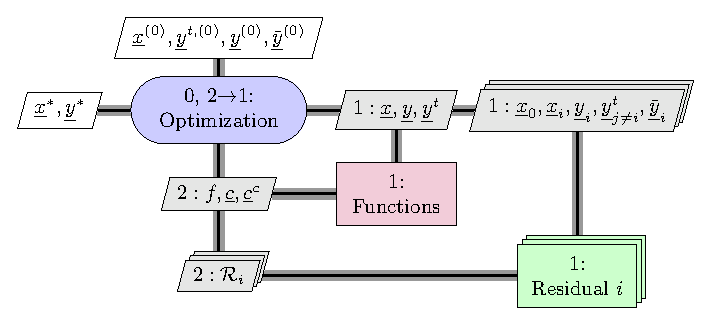
\includegraphics[keepaspectratio, width=0.8\textwidth]{images/app_mdo/AAO}
	\caption{xDSM diagram for the AAO problem.}
	\label{fig:aao_arch}
\end{figure}

In practice, the AAO problem is never solver in this form because the consistency constraints can be easily eliminated without comprimising the algorithm. 
More in general, different architectures can be deduced from Problem~\eqref{eq:aao_prob}, depending on which equality constraint groups are eliminated. 
They are three: the simultaneous analysis and design SAND, the individual discipline feasible IDF and the multidisciplinary feasible MDF architecture, that have been well known in literature for a long time~\cite{bib:kroo_1997, bib:balling, bib:haftka_1985, bib:schmit_1978}. 

The SAND architecture is obtained removing the consistency constraints by introducing a single group of coupling variables to replace the separate target and response groups. 
This change yields to the following formulation:
\begin{equation}
\label{eq:sand_prob}
\begin{array}{l l l}
\textrm{minimize } & f_0\left(\underline{x},\underline{y}\right) & \\
\textrm{with respect to } & \underline{x}, \underline{y}, \bar{y} & \\
\textrm{subject to } & \underline{c}_0\left(\underline{x}, \underline{y}\right)\geq 0 & \\
& c_i\left(x_0, x_i, y_i\right) \geq 0 & \textrm{for } i=1,\cdots,N \\
& \mathcal{R}_i(x_0,x_i,y^t_{j\neq i}, \bar{y}_i, y_i) = 0 & \textrm{for } i=1,\cdots,N \\					 
\end{array}
\end{equation}
The corresponding xDSM diagram is shown in Fig.~\ref{fig:sand_arch}.
\begin{figure}[!h]
	\centering
	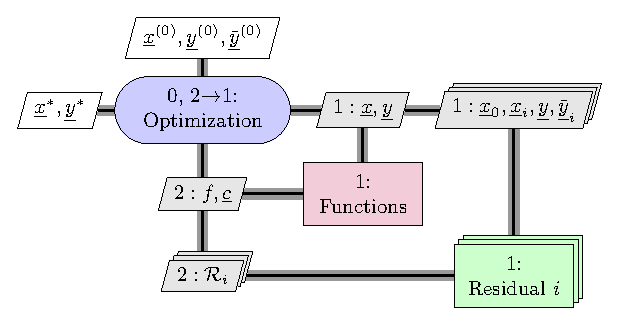
\includegraphics[keepaspectratio, width=0.8\textwidth]{images/app_mdo/SAND}
	\caption{xDSM diagram for the SAND architecture.}
	\label{fig:sand_arch}
\end{figure}
The main feature of the SAND architecture is that, since there is no need to solve any discipline analysis at each iteration, the problem can be solved quickly by letting the optimizer explore regions infeasible with respect to the analysis constraints $\mathcal{R}_i$. 
However, it presents two main issues. 
First, despite there are no more consistency constraint, the formulation still requires all state variables and discipline analysis equations, and then problem size at quick convergence can be issued in pratice. 
Second, discipline analysis equations are treated explicitly and then residual values, and their derivatives in case of a gradient-based formulation, need to be available at the optimizer level. 
This means that, rather than computing $y_i$ and $\bar{y}_i$, each discipline takes predetermined values of these parameters and returns the residuals $\mathcal{R}_i$. 
Often, in engineering, softwares for disciplines are ``black box'' that hide residuals and state variables and return directly coupling variables; also they are not accessible to users for editing. 
This limits the field application of SAND architecture. 

To solve the issue, the discipline analysis constraints can be eliminated from Problem~\eqref{eq:aao_prob}, yielding to the IDF architecture. 
The new statement is:
\begin{equation}
\label{eq:idf_prob}
\begin{array}{l l l}
\textrm{minimize } & f_0\left(\underline{x},\underline{y}\left(\underline{x}, \underline{y}^t\right)\right) & \\
\textrm{with respect to } & \underline{x}, \underline{y}^t & \\
\textrm{subject to } & \underline{c}_0\left(\underline{x}, \underline{y}\left(\underline{x}, \underline{y}^t\right)\right)\geq 0 & \\
& c_i\left(x_0, x_i, y_i\left(\underline{x}_0, \underline{x}_i, \underline{y}_{i\neq j}^t\right)\right) \geq 0 & \textrm{for } i=1,\cdots,N \\
& c_i^c = y_i^t - y_i\left(\underline{x}_0, \underline{x}_i, \underline{y}_{i\neq j}^t\right) = 0 & \textrm{for } i=1,\cdots,N \\	
\end{array}
\end{equation}
Diagram for IDF architecture is depicted in Fig.~\ref{fig:idf_arch}. 
\begin{figure}[!h]
	\centering
	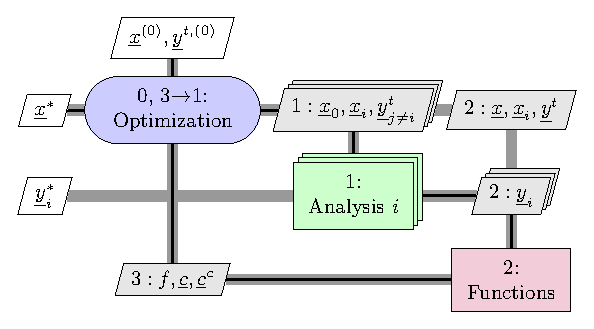
\includegraphics[keepaspectratio, width=0.8\textwidth]{images/app_mdo/IDF}
	\caption{xDSM diagram for the IDF architecture.}
	\label{fig:idf_arch}
\end{figure}

The main consequence of this reformulation is the removal of all the state variables and discipline analysis. 
IDF architecture finally allows the possibility to use "black box" analyses for the disciplines, enlarging the field of application of SAND, and it also enables parallel computation. 
Despite the IDF problem is smaller than the SAND, it needs in any case the consistency constraint and thus does not solve the first SAND issue, that is the large size. 
This can be a relevant point in the procedure when the problem is really large, \textit{i.e.} as in the high fidelity optimization. 
Also, when the gradient-based are used, an accurate gradients calculation, needed for the optimal solution, can be very expensive in term of computational cost~\cite{bib:hwang_omdao}, making the application of this architecture sometime unfeasible without a large amount of computational resources available. 

To still reduce the problem size, the last modification that can be done is to remove from Problem~\eqref{eq:idf_prob} also the consistency constraints, or both the consistency constraints and the residual constraints from Problem~\eqref{eq:aao_prob}, obtaining the MDF architecture:
\begin{equation}
\label{eq:mdf_prob}
\begin{array}{l l l}
\textrm{minimize } & f_0\left(\underline{x},\underline{y}\left(\underline{x}, \underline{y}\right)\right) & \\
\textrm{with respect to } & \underline{x} & \\
\textrm{subject to } & \underline{c}_0\left(\underline{x}, \underline{y}\left(\underline{x}, \underline{y}\right)\right)\geq 0 & \\
& c_i\left(x_0, x_i, y_i\left(\underline{x}_0, \underline{x}_i, \underline{y}_{i\neq j}^t\right)\right) \geq 0 & \textrm{for } i=1,\cdots,N \\
\end{array}
\end{equation}
The main consequence of the reformulation is that MDF requires a consistent set of coupling variables to be returned to the optimizer every time the objective and constraint functions are re-evaluated. 
In practice, it has to perform a fully MDA at each iteration. 
The xDSM diagram for the MDF architecture is shown in Fig.~\ref{fig:mdf_arch}, considering three disciplines. 
\begin{figure}[!h]
	\centering
	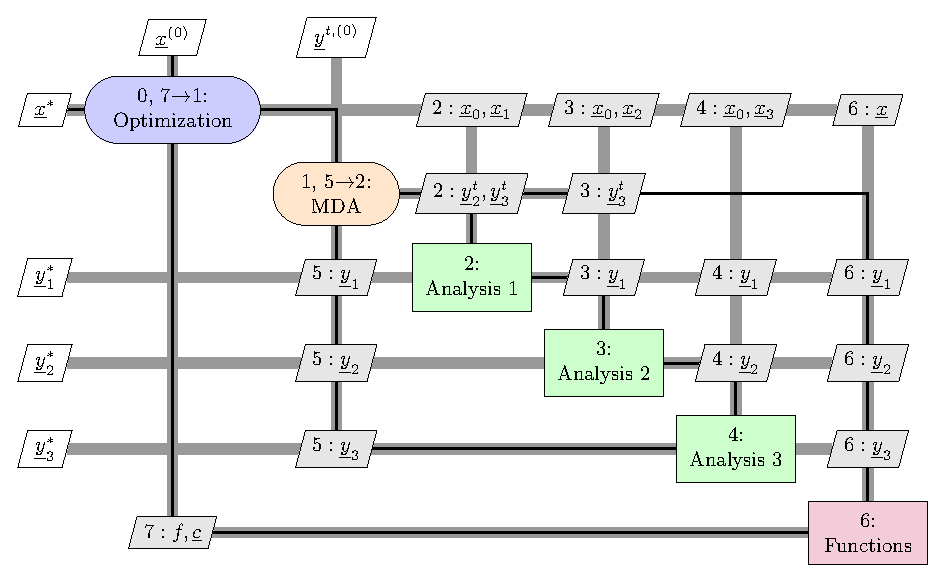
\includegraphics[keepaspectratio, width=0.8\textwidth]{images/app_mdo/MDF}
	\caption{xDSM diagram for the MDF architecture.}
	\label{fig:mdf_arch}
\end{figure}

Because of the MDA to be solved at each iteration, MDF shows a slower convergence rate (see also Fig.~\ref{fig:mdo_benchmarking}). 
It can be accelerated using proper algorithm for the MDA, like the Gauss-Seidel~\cite{bib:bloebaum} or the Newton~\cite{bib:kennedy} methods, or adding preconditioners to the linear system~\cite{bib:leveque_partial_equation}. 
Parallel computation also depends on the algorithm for the MDA, since some of them are sequential and do not allows parallelization. 

The main advantage of the MDF is the reduced size of the problem, since only objective function, design variables and constraints are under the control of the optimizer. 
Also, it always returns a point that satisfies the consistency constraints, even if the optimization terminates earlier, because of the MDA.
This feature is of main interest in aircraft design, since it is still possible to get a tradeoff between final design and design variables, even if the optimization is not reached. 
However, it is to remarl that only the consistency is assured, but not the feasibility: nothing ensures, indeed, tha also design constraints are satisfied. 
This last condition can be ensured chosing methods that maintain feasible design point during the iterations: methods to keep the feasible direction have been developed at that scope~\cite{bib:vanderplaats}. 
It is to note that the robust sequential quadratric programming methods, which represent a large category for gradient-based optimization, do not ensure the feasibility~\cite{bib:snopt, bib:slsqp}. 

The main drawback is the requirement of a converged MDA for each iteration. 
In case derivatives are needed, their calculation is more complicated than the IDF, because they need to be feasible with respect to all disciplines, and not only discipline feasible as in the IDF. 
The work of Martins and Hwang contains a set of methods to compute efficiently derivatives, to address the problem both in IDF and MDF architectures~\cite{bib:hwang_unif}

At this point, it has to emphasize that, despite the architectures are changing because of the elements added or removed, the MDO problem is always the same. 
Furthemore, it has the same set of optimal solution. 

As said at the beginning, the distributed architectures are beyond the interest of this work: for completeness a classification of them is reported in Fig.~\ref{fig:mdo_arch_summary}; more information can be found in the work of Martins and Lambe~\cite{bib:martins_mdo}. Just note that the distributed formulations are deduced from the IDF and MDF architectures. 
\begin{figure}[!h]
	\centering
	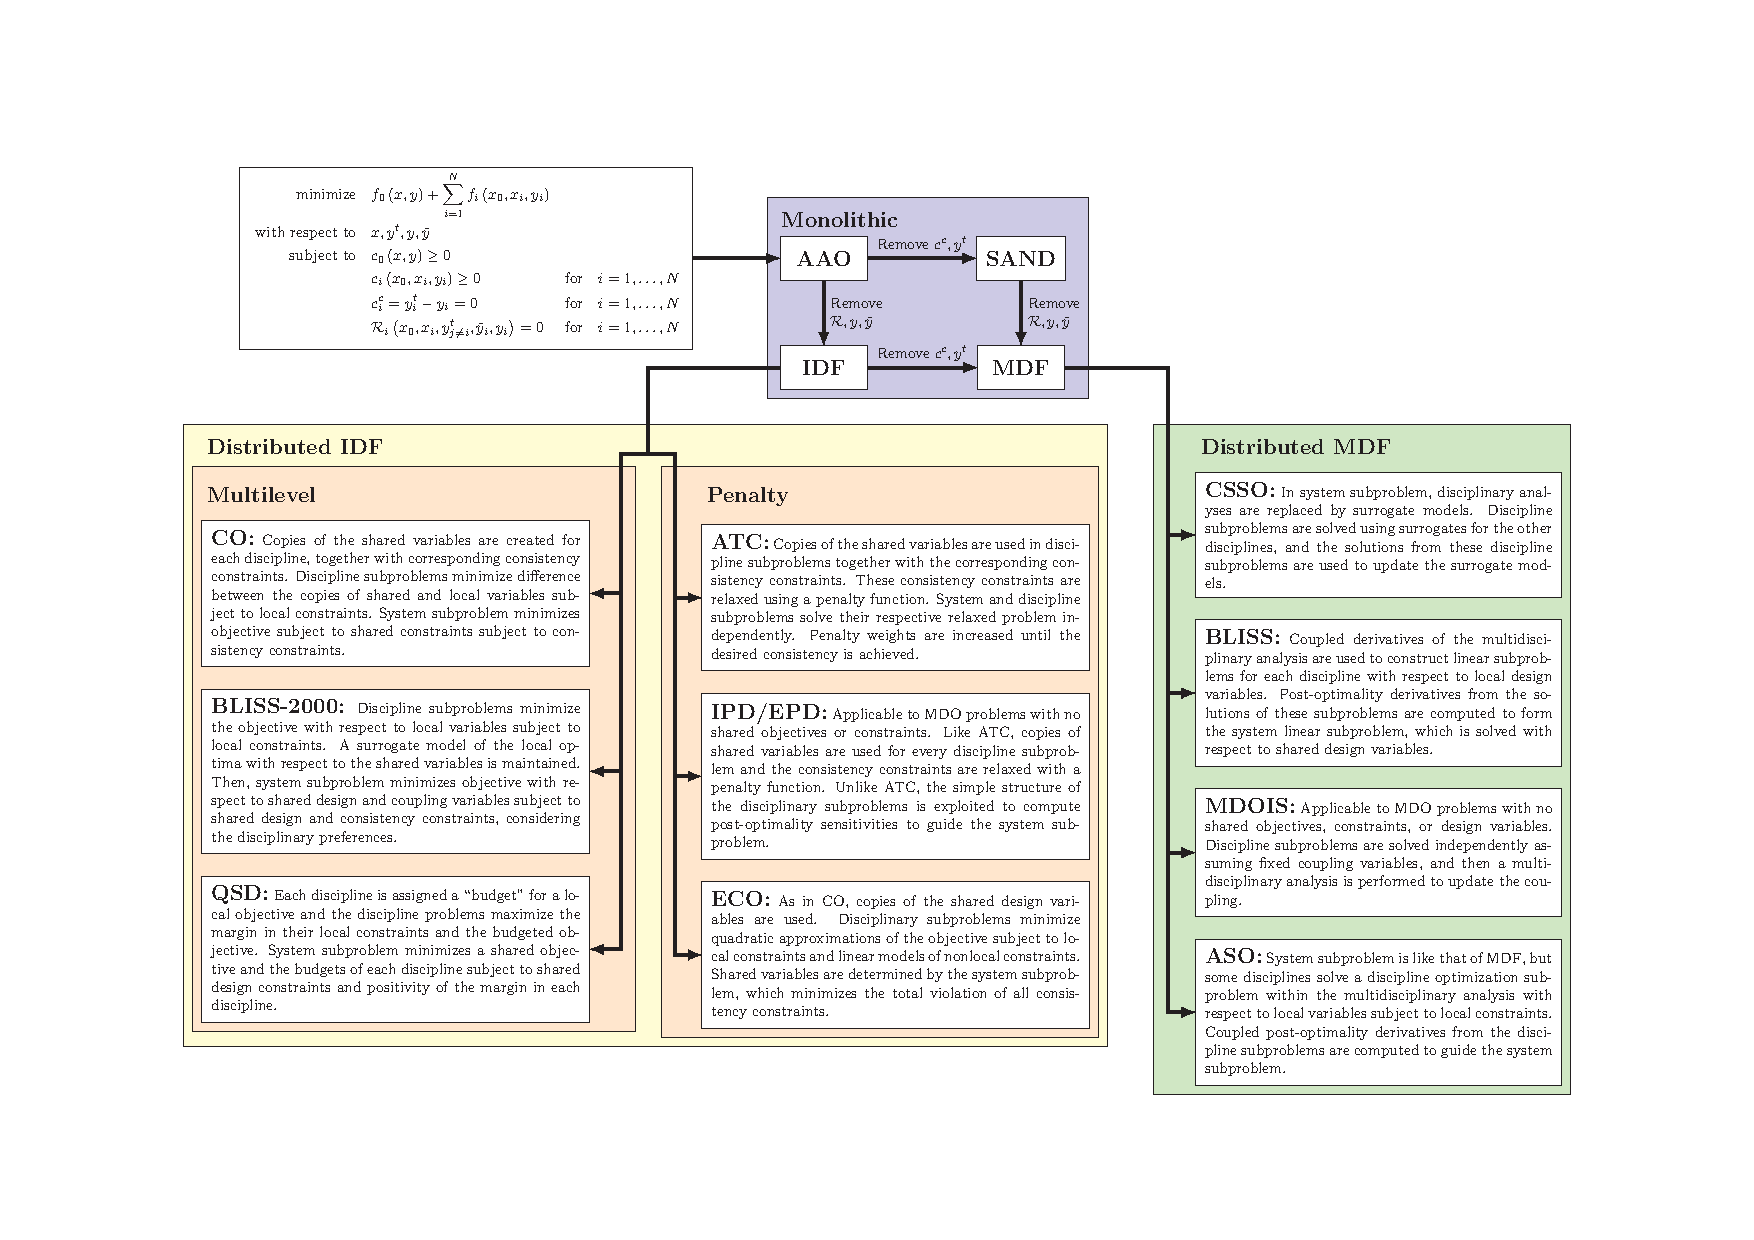
\includegraphics[keepaspectratio, width=1.3\linewidth, angle=90]{images/app_mdo/mdo_arch_summary}
	\caption{Summary of MDO architectures~\cite{bib:martins_mdo}.}
	\label{fig:mdo_arch_summary}
\end{figure}